% !TeX program = pdflatex
% Main manuscript for submission to Frontiers of Computer Science.
\documentclass[research]{fcs}

\usepackage{subfig}
\usepackage{algorithm}
\usepackage{algorithmicx}
\usepackage{algpseudocode}
\usepackage{listings}
\usepackage{tikz}
\usetikzlibrary{arrows.meta,calc,fit,positioning,shapes.geometric}

\title{Accelerating Latency-Bound EKF Fusion Positioning for Downhole Traction Robots via Kernel Fusion, Mixed Precision, and Multi-Trajectory Parallelism}
\shorttitle{GPU Acceleration of Downhole Traction Robot Positioning}

% TODO: Replace the author, affiliation, and correspondence placeholders.
\author[1,+]{First~Author}
\author[1]{Second~Author}
\address[1]{Department, University, City Postal Code, China}
\corremail{corresponding.author@example.com}

\fcssetup{
  received = {month dd, yyyy},
  accepted = {month dd, yyyy},
  article-id = {1},
  first-page = {1},
}

\begin{abstract}
Extended Kalman filter (EKF)-based multi-sensor fusion is widely used to evaluate positioning algorithms for robots operating without reliable external positioning. In simulations of a downhole traction robot operating in a cased horizontal well, the estimator processes a long sensor sequence through tightly dependent SINS propagation and EKF correction steps. Its small matrices and fine-grained operators produce a latency-bound GPU workload: a direct tensor implementation expands each filter step into hundreds of dependent kernels and leaves most streaming multiprocessors idle. This paper presents a three-axis GPU acceleration framework for this workload. First, a Triton whole-scan kernel fuses the complete recursive trajectory, retains the recurrent navigation and filter state on chip, and replaces the general innovation solve with an analytical small-matrix inverse. Second, component-aware specialization separates sensor input, recurrent computation, and dot-product precision to control long-horizon numerical error while reducing instruction and storage costs. Third, independent simulation trajectories are mapped to CUDA blocks to expose batch-level parallelism without changing the temporal order within each filter. On a Hopper-class GPU, whole-scan fusion in fp64 provides an $8.8\times$ speedup over the CPU reference, while the fused fp32 implementation reaches approximately $2.43\times10^{5}$ filter steps per second, corresponding to a $130\times$ single-trajectory speedup with sub-millimeter deviation from the fp64 trajectory. Multi-trajectory execution scales aggregate throughput to $4.63\times10^{7}$ filter steps per second before register-limited saturation. These results show how execution granularity, numerical representation, and outer-loop parallelism can be coordinated for long-horizon recursive state-estimation simulation.
\end{abstract}
\keywords{}
\ExplSyntaxOn
\tl_clear:N \l__fcs_keywords_tl
\ExplSyntaxOff

\begin{document}

\section{Introduction}
\label{sec:introduction}

Embodied artificial intelligence (AI) is extending autonomous machines from structured, instrumented spaces into physical environments with uncertain contacts, limited visibility, and unreliable external positioning~\cite{liu2025embodied-survey}. A robot must maintain an estimate of its pose, velocity, and internal state while it perceives the environment, plans a motion, and applies control. Deep-space vehicles, subterranean platforms, legged robots, and autonomous vehicles use different sensors and motion models, yet their local state-estimation loops repeatedly propagate inertial information and correct it with intermittent observations through recursive Bayesian estimation~\cite{he2024legged-state,ou2024leg-kilo}. The quality and timeliness of this loop determine how reliably the rest of the perception--action system can operate.

This requirement is especially visible in embodied-AI systems~\cite{embodied-ai-survey}. Humanoids and quadrupeds combine inertial, kinematic, contact, and visual measurements at high update rates; a local extended Kalman filter (EKF) or error-state filter often provides the deterministic propagation layer even when a separate mapping system supplies global consistency. Consistent fusion of leg kinematics and inertial measurements has been demonstrated for legged robots~\cite{bloesch2012}, while the DARPA Subterranean Challenge shows how localization, mapping, and navigation must remain tightly coupled when robots operate in underground environments~\cite{cerberus2022}. The same systems increasingly depend on large simulation campaigns that vary contact conditions, sensor noise, terrain, and control parameters. GPU-native simulators such as Isaac Gym make thousands of robot environments executable concurrently~\cite{isaacgym2021}, which raises the throughput requirements of every repeated state-estimation loop in the simulation pipeline.

Downhole traction robots provide a concrete and demanding instance of this broader embodied-autonomy problem. These robots actively convey coiled tubing, wireline, and attached tools through highly deviated and horizontal wells, where gravity, friction, and long constrained passages make passive delivery unreliable. Recent field deployments have demonstrated their use in horizontal-well intervention, logging, perforation, and zonal-isolation operations~\cite{he2020downhole-tractor,chawla2024tractor-glide}. As illustrated in \Cref{fig:downhole-tractor}, a surface unit deploys the toolstring through the wellbore while the tractor provides active conveyance along the horizontal section. In the cased horizontal well considered in this study, high temperature and pressure, corrosion, deposits, local deformation, and obstructions can perturb wheel--wall contact and induce slip or short-lived odometry disturbances. Reliable operation therefore requires continuous fusion of inertial and traction measurements to estimate the robot state and suppress accumulated drift. Before deployment, large simulation campaigns are needed to evaluate sensor noise, slip events, obstacle-induced disturbances, and filter parameters over long trajectories, making downhole traction robot positioning not only a state-estimation problem but also a computationally intensive simulation workload.

\begin{figure}[!t]
  \centering
  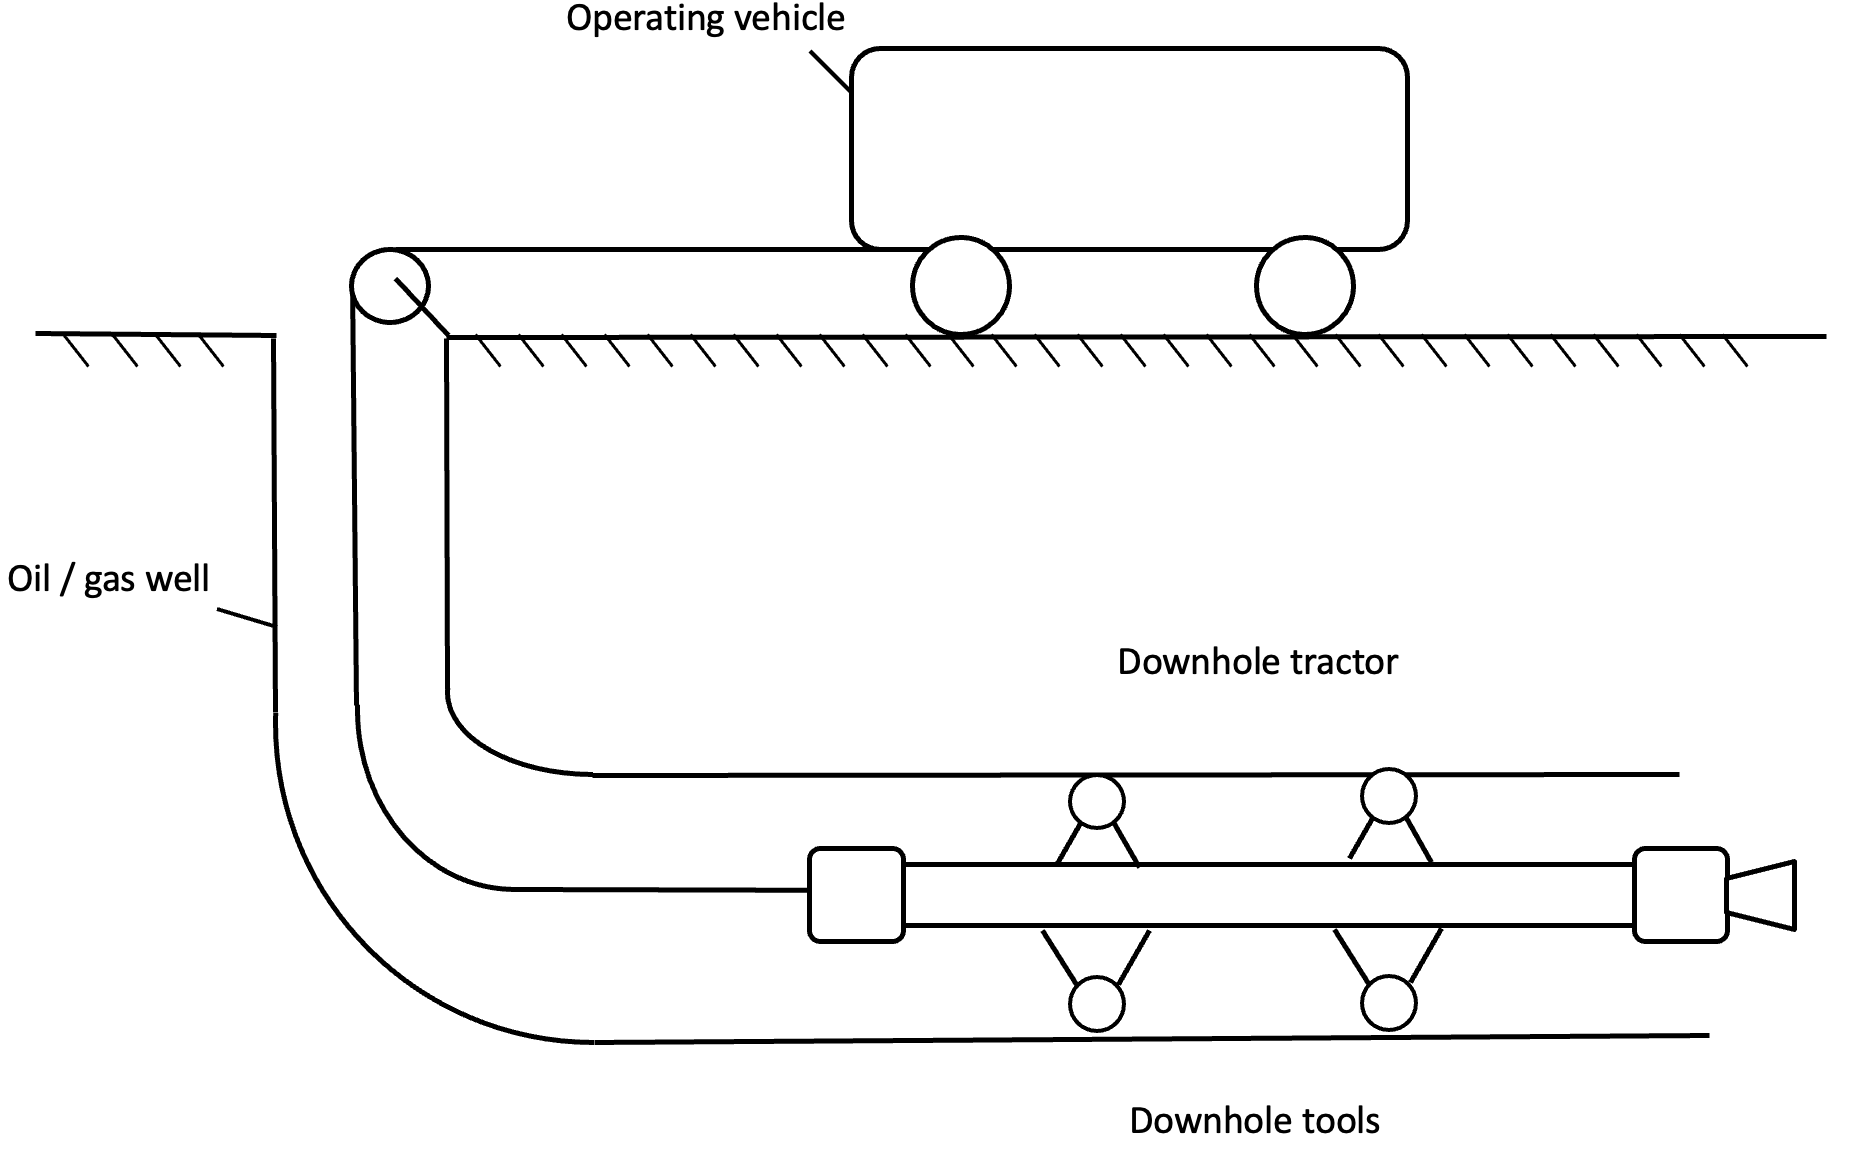
\includegraphics[width=\linewidth]{../downhole_tractor.png}
  \caption{Schematic of a downhole traction robot conveying a toolstring into the horizontal section of an oil or gas well.}
  \label{fig:downhole-tractor}
\end{figure}

The resulting estimator has an execution pattern that differs from the large, throughput-oriented matrix workloads commonly used to showcase GPUs. Each update is a small numerical operation embedded in a long dependency chain, and a direct tensor implementation fragments the computation into many fine-grained device operations. Repeated launches, synchronization, and movement of recurrent state can dominate arithmetic, leaving much of the accelerator underutilized and causing a straightforward GPU port to underperform a CPU implementation. These characteristics motivate an implementation study centered on launch overhead, on-chip state locality, numerical precision, and independent trajectories available at the simulation level.

We develop a GPU acceleration framework for this workload. Operator fusion removes fragmented execution and intermediate-state traffic; component-aware precision matches numerical requirements to GPU instruction throughput; and multi-trajectory parallelism fills otherwise idle SMs while preserving the temporal dependency within each trajectory. The main contributions are as follows:

\begin{itemize}
  \item We diagnose the execution behavior of SINS/EKF simulation and develop a progressive fusion path culminating in a single Triton mega-kernel that keeps the recurrent filter state on chip and executes a complete trajectory with minimal device dispatch.
  \item We establish a component-aware precision strategy for recursive filtering and evaluate the performance and long-horizon accuracy of fp64, fp32, reduced-precision input, bfloat16, and TensorFloat-32 paths, including failure cases caused by error accumulation.
  \item We map independent trajectories to CUDA blocks and derive a scaling model that relates batch throughput to accelerator occupancy and register pressure, enabling high-throughput Monte Carlo and parameter-sweep simulation.
\end{itemize}

The remaining sections of this paper are organized as follows. \Cref{sec:background} introduces the positioning model and its computational structure. \Cref{sec:motivation} presents the profiling evidence and optimization requirements. \Cref{sec:methodology} describes the acceleration framework. \Cref{sec:evaluation} evaluates performance, accuracy, and scalability. \Cref{sec:related-work} discusses related work, and \Cref{sec:conclusion} concludes the paper.

\section{Background}
\label{sec:background}

\subsection{Downhole Traction Robot Positioning}
\label{subsec:positioning-background}

Downhole traction robots for coiled-tubing operations actively convey tubing and payloads through highly deviated and horizontal wells. The deployment configuration in \Cref{fig:downhole-tractor} shows the tractor moving with the toolstring while its drive elements maintain contact with the well wall. This study considers operation inside a cased horizontal well, where the available space is narrow and absolute positioning signals are generally unavailable. High temperature, pressure, corrosion, well-wall deformation, deposits, and local obstacles can change the contact conditions between the robot and the casing. These effects can introduce wheel slip and short-duration disturbances while the robot performs traction, logging, inspection, or other downhole operations. A positioning system must therefore maintain a local state estimate over a long constrained motion and remain useful when an individual measurement becomes unreliable.

The simulated platform uses a three-axis inertial measurement unit (IMU) and two wheel odometers. Gyroscope and accelerometer measurements support high-rate propagation of attitude, velocity, and position, but their biases cause the propagated solution to drift over time. The odometers provide an independent estimate of traveled distance and can correct this drift, while disagreement between the two odometers or between odometry and inertial propagation provides a signal for detecting local disturbances. The fusion system uses these complementary measurements in a local navigation frame whose origin and initial attitude are set during initialization.

The casing geometry supplies additional information about feasible robot motion. During nominal traction, displacement is dominated by the direction of the well axis, whereas sustained lateral or radial velocity is inconsistent with the confined workspace. These motion constraints improve local observability when absolute position is unavailable. They cannot, however, be treated as uniformly reliable: wheel slip, asymmetric traction, and obstacle contact can produce transient measurements that violate the nominal motion pattern. The estimator must therefore combine continuous inertial propagation with measurement selection, using the available odometry information without allowing a short-lived contact disturbance to corrupt the full trajectory.

\subsection{SINS/EKF Fusion Model}
\label{subsec:ekf-model}

The simulation follows a strapdown inertial navigation system (SINS) with an error-state extended Kalman filter. At sample $k$, the SINS first updates the quaternion attitude from the angular-rate measurement, converts the measured specific force from the body frame to the navigation frame, subtracts gravity, and integrates velocity and position. Quaternion normalization is applied after each update to keep the attitude representation bounded.

The SINS state is maintained as a nominal navigation solution, while the EKF represents only small deviations from that solution. This error-state formulation separates the nonlinear integration of attitude and motion from the locally linear uncertainty update. It also supports closed-loop correction: after the EKF estimates the navigation errors, the nominal position, velocity, and attitude are corrected and the corresponding error coordinates are reset. Sensor biases remain part of the estimated state because even small bias errors can accumulate during a long period without an external position reference.

The EKF estimates the error of the nominal SINS state. Its 15-dimensional error vector is
\begin{equation}
  \mathbf{x}_k =
  [\delta\mathbf{p}_k^{\mathsf T},
   \delta\mathbf{v}_k^{\mathsf T},
   \boldsymbol{\phi}_k^{\mathsf T},
   \boldsymbol{\varepsilon}_k^{\mathsf T},
   \boldsymbol{\nabla}_k^{\mathsf T}]^{\mathsf T}
  \in \mathbb{R}^{15},
  \label{eq:error-state}
\end{equation}
where the five three-dimensional components represent position error, velocity error, attitude error, gyroscope bias, and accelerometer bias, respectively.

The linearized transition matrix is constructed from the current attitude, specific force, angular rate, and sampling interval. The covariance and error state are then propagated and corrected through the standard EKF prediction and measurement update:
\begin{align}
  \mathbf{x}_{k}^{-} &= \mathbf{F}_k\mathbf{x}_{k-1}, \\
  \mathbf{P}_{k}^{-} &= \mathbf{F}_k\mathbf{P}_{k-1}\mathbf{F}_k^{\mathsf T}+\mathbf{Q}_k, \\
  \mathbf{K}_k &= \mathbf{P}_{k}^{-}\mathbf{H}_k^{\mathsf T}
  (\mathbf{H}_k\mathbf{P}_{k}^{-}\mathbf{H}_k^{\mathsf T}+\mathbf{R}_k)^{-1}, \\
  \mathbf{x}_k &= \mathbf{x}_{k}^{-}+\mathbf{K}_k
  (\mathbf{z}_k-\mathbf{H}_k\mathbf{x}_{k}^{-}), \\
  \mathbf{P}_k &= (\mathbf{I}-\mathbf{K}_k\mathbf{H}_k)\mathbf{P}_{k}^{-}.
  \label{eq:ekf-update}
\end{align}

Here, $\mathbf{F}_k$ is the linearized state-transition matrix, $\mathbf{P}_k$ is the error covariance, and $\mathbf{Q}_k$ models process uncertainty. The observation matrix $\mathbf{H}_k$ maps the error state into the currently available measurement space, while $\mathbf{R}_k$ represents measurement uncertainty. The matrix inverted in the gain calculation is the innovation covariance. Although its dimension is small in this application, its value changes with the propagated covariance and the accepted measurement set at every sample.

The measurement model uses the odometry displacement together with lateral and radial velocity constraints when the odometry consistency test accepts both channels. If a channel is judged to be affected by a local obstacle, the update uses only the remaining reliable constraints. The estimated position, velocity, and attitude errors are fed back to the nominal SINS state, and the error state is reset before the next sample. This feedback loop makes every update depend on the state and covariance produced at the previous sample.

\subsection{Computational Characteristics}
\label{subsec:workload-characteristics}

The overall computation is summarized in \Cref{fig:computational-flow}. The resulting workload is a long sequential scan of sensor samples. Each step combines quaternion and vector operations with covariance propagation, a small innovation calculation, and several products involving matrices whose logical dimensions are no larger than $15\times15$. The arithmetic intensity of an individual step is consequently modest, while the recurrent state and covariance must remain available for the next step. Temporal parallelism within one trajectory is therefore limited by the estimator semantics.

\begin{figure}[!t]
  \centering
  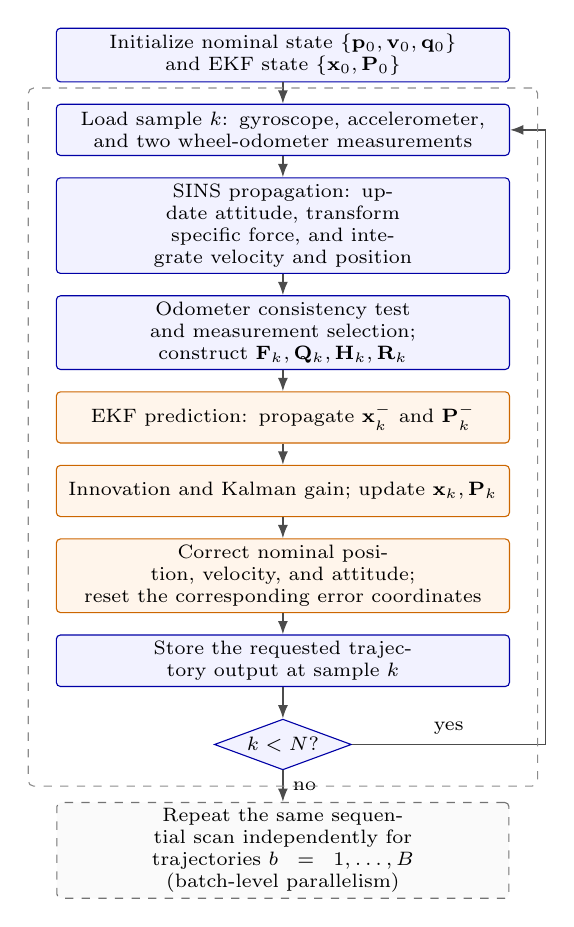
\begin{tikzpicture}[
      node distance=2.7mm,
      font=\scriptsize,
      flow/.style={draw=blue!65!black, rounded corners=1.5pt,
        fill=blue!5, align=center, minimum height=6.5mm,
        text width=5.6cm, inner sep=2.2pt},
      update/.style={flow, draw=orange!80!black, fill=orange!8},
      decision/.style={diamond, draw=blue!65!black, fill=blue!5,
        align=center, aspect=2.7, inner sep=1.2pt},
      note/.style={draw=black!55, dashed, rounded corners=1.5pt,
        fill=black!2, align=center, minimum height=6mm,
        text width=5.6cm, inner sep=2pt},
      arrow/.style={-{Latex[length=1.7mm]}, semithick, draw=black!70}
    ]
    \node[flow] (init) {Initialize nominal state $\{\mathbf{p}_0,\mathbf{v}_0,\mathbf{q}_0\}$\\and EKF state $\{\mathbf{x}_0,\mathbf{P}_0\}$};
    \node[flow, below=of init] (load) {Load sample $k$: gyroscope, accelerometer,\\and two wheel-odometer measurements};
    \node[flow, below=of load] (sins) {SINS propagation: update attitude, transform\\specific force, and integrate velocity and position};
    \node[flow, below=of sins] (select) {Odometer consistency test and measurement selection;\\construct $\mathbf{F}_k,\mathbf{Q}_k,\mathbf{H}_k,\mathbf{R}_k$};
    \node[update, below=of select] (predict) {EKF prediction: propagate $\mathbf{x}_k^{-}$ and $\mathbf{P}_k^{-}$};
    \node[update, below=of predict] (correct) {Innovation and Kalman gain; update $\mathbf{x}_k,\mathbf{P}_k$};
    \node[update, below=of correct] (feedback) {Correct nominal position, velocity, and attitude;\\reset the corresponding error coordinates};
    \node[flow, below=of feedback] (store) {Store the requested trajectory output at sample $k$};
    \node[decision, below=4.0mm of store] (next) {$k<N$?};
    \node[note, below=4.0mm of next] (batch) {Repeat the same sequential scan independently for\\trajectories $b=1,\ldots,B$ (batch-level parallelism)};

    \draw[arrow] (init) -- (load);
    \draw[arrow] (load) -- (sins);
    \draw[arrow] (sins) -- (select);
    \draw[arrow] (select) -- (predict);
    \draw[arrow] (predict) -- (correct);
    \draw[arrow] (correct) -- (feedback);
    \draw[arrow] (feedback) -- (store);
    \draw[arrow] (store) -- (next);
    \draw[arrow] (next) -- node[right, font=\scriptsize] {no} (batch);
    \coordinate (returntop) at ([xshift=4.5mm]load.east);
    \coordinate (returnbottom) at (next.east -| returntop);
    \draw[arrow] (next.east) -- node[above, font=\scriptsize] {yes}
      (returnbottom) |- (load.east);

    \node (scanbox) [draw=black!45, dashed, rounded corners=2pt,
      fit=(load)(next), inner xsep=3.5mm, inner ysep=2.0mm] {};
  \end{tikzpicture}
  \caption{Overall computational flow of the SINS/EKF positioning simulation. Operations within one trajectory follow a loop-carried dependency, whereas different trajectories have independent recurrent states and can be evaluated in parallel.}
  \label{fig:computational-flow}
\end{figure}

The covariance alone contains 225 logical elements, yet this state is still too small to provide the spatial parallelism of a large dense matrix operation. Moreover, the matrices used at a given sample are assembled from the current navigation state and measurement-validity decision rather than reused unchanged across the sequence. The workload therefore alternates small matrix products with quaternion normalization, coordinate transforms, scalar tests, and feedback operations. Its defining feature is not the cost of any individual operator, but the repeated execution of this heterogeneous operator chain under a loop-carried dependency.

The simulation nevertheless exposes a second form of parallelism. Trajectories generated with different noise realizations, obstacle configurations, or filter parameters do not share state and can be evaluated independently. Increasing the trajectory length adds sequential work, whereas increasing the number of trajectories adds independent work. The workload thus combines a sequential dependency along each trajectory with batch-level independence across trajectories. This combination defines the execution target for the optimization methods developed in the remaining sections of the paper. For fixed-shape kernel implementations, the logical filter matrices may be stored in padded $16\times16$ tiles without changing the 15-state model.

\section{Motivation}
\label{sec:motivation}

\subsection{Fine-Grained EKF Execution Is Latency-Bound}
\label{subsec:motivation-latency}

The CPU fp64 implementation processes approximately 1,866 filter steps per second and serves as the numerical reference. Moving the same tensor-level computation directly to the GPU does not produce a corresponding speedup. Each EKF step contains a dependent chain of tensor construction, element-wise arithmetic, trigonometric functions, and small matrix operations. The eager implementation expands this modest amount of arithmetic into roughly 531 CUDA kernel launches per step. As a result, dispatch, synchronization, and recurrent-state transfers occupy a substantial part of the execution time.

Device measurements confirm that the baseline is latency-bound. A single trajectory activates only a small portion of the GPU, and its measured SM throughput is approximately $0.27\%$. The launch cost of a general-purpose small-matrix kernel can approach or exceed the cost of its arithmetic. CUDA Graph replay reduces repeated host dispatch, but the captured graph still executes the fine-grained dependent kernels and transfers state between them. These observations motivate a larger execution scope that can preserve recurrent data across filter steps and eliminate fragmented device execution.

\begin{table}[H]
  \centering
  \caption{Representative characteristics of the baseline positioning workload.}
  \label{tab:baseline-characteristics}
  \begin{tabular}{@{}lr@{}}
    \toprule
    Characteristic & Value \\
    \midrule
    Trajectory length & 166,667 steps \\
    EKF state dimension & 15 \\
    Maximum logical matrix size & $15\times15$ \\
    Naive kernels per step & approximately 531 \\
    CPU fp64 throughput & 1,866 steps/s \\
    Naive GPU SM throughput & approximately 0.27\% \\
    \bottomrule
  \end{tabular}
\end{table}

\subsection{Precision Choices Have Unequal Numerical and Hardware Effects}
\label{subsec:motivation-precision}

Uniformly changing the precision of the estimator overlooks the different roles of its components. Sensor samples are noisy external inputs that are consumed once, whereas position, velocity, attitude, error state, and covariance are carried through the complete trajectory. Rounding in these recurrent quantities can accumulate through repeated propagation and feedback. Accuracy measured for an isolated filter step is therefore insufficient to determine whether a reduced-precision configuration is acceptable over a long simulation.

Lower nominal precision also does not guarantee lower execution time. TensorFloat-32 and Tensor Core paths may require conversion, padding, and scheduling work that is difficult to amortize for the small matrices in this estimator. Storage precision, recurrent arithmetic, and matrix-multiplication mode consequently present different accuracy and performance trade-offs. This behavior motivates component-level precision choices evaluated with both hardware measurements and complete-trajectory numerical error.

\subsection{Independent Trajectories Supply Device-Level Parallelism}
\label{subsec:motivation-trajectories}

The state and covariance at time $k$ depend on the result at time $k-1$, which limits temporal parallelism within one trajectory. Increasing the tile size or assigning more threads to an individual small matrix product cannot create work along this dependency chain. After fusion, one trajectory is processed by one block and still leaves most SMs without useful work, so reducing single-trajectory latency alone cannot fully utilize the device.

Simulation campaigns naturally provide an outer parallel dimension. Different noise realizations, obstacle configurations, and filter parameters produce independent trajectories with no shared recurrent state. Mapping these trajectories to separate blocks preserves the original update order within every filter while increasing aggregate device utilization. Scaling eventually becomes limited by the number of SMs and by register-constrained block residency. Together, the three observations above lead to whole-scan kernel fusion, component-aware precision, and multi-trajectory parallelism, which are developed in the next section.

\section{Methodology}
\label{sec:methodology}

\subsection{Overview}
\label{subsec:method-overview}

The proposed framework treats one positioning trajectory as a recursive scan over $N$ sensor samples. At every step, the scan reads the current IMU and odometer measurements, propagates the nominal SINS state, performs the EKF prediction and correction, feeds the estimated error back to the nominal state, and carries the resulting state and covariance to the next step. For a batch of $B$ simulations, the input and output tensors contain an additional trajectory dimension, while the recursive state of each trajectory remains private.

As summarized in \Cref{fig:design-overview}, we optimize this scan along three complementary axes. Whole-scan kernel fusion changes the execution granularity and keeps recurrent data close to the arithmetic that consumes it. Component-aware precision specialization changes the representation of sensor data, recurrent state, and matrix products according to their numerical roles. Multi-trajectory parallelism maps independent scans to different CUDA blocks and thereby supplies work across the device. Fusion primarily reduces dispatch and data-movement latency, precision specialization reduces critical-path instruction and storage cost, and trajectory mapping improves device-level utilization. Their mechanisms do not require a change to the SINS/EKF equations and can therefore be composed in one implementation.

All transformations preserve the ordering of propagation, measurement update, and feedback within a trajectory. We use the CPU fp64 implementation as the semantic reference and validate each transformation with state differences and axis-wise positioning RMSE. Batch implementations additionally compare repeated identical trajectories to detect unintended inter-block state sharing. These checks are part of the design process; the corresponding quantitative results are reported in \Cref{sec:evaluation}.

\begin{figure*}[!t]
  \centering
  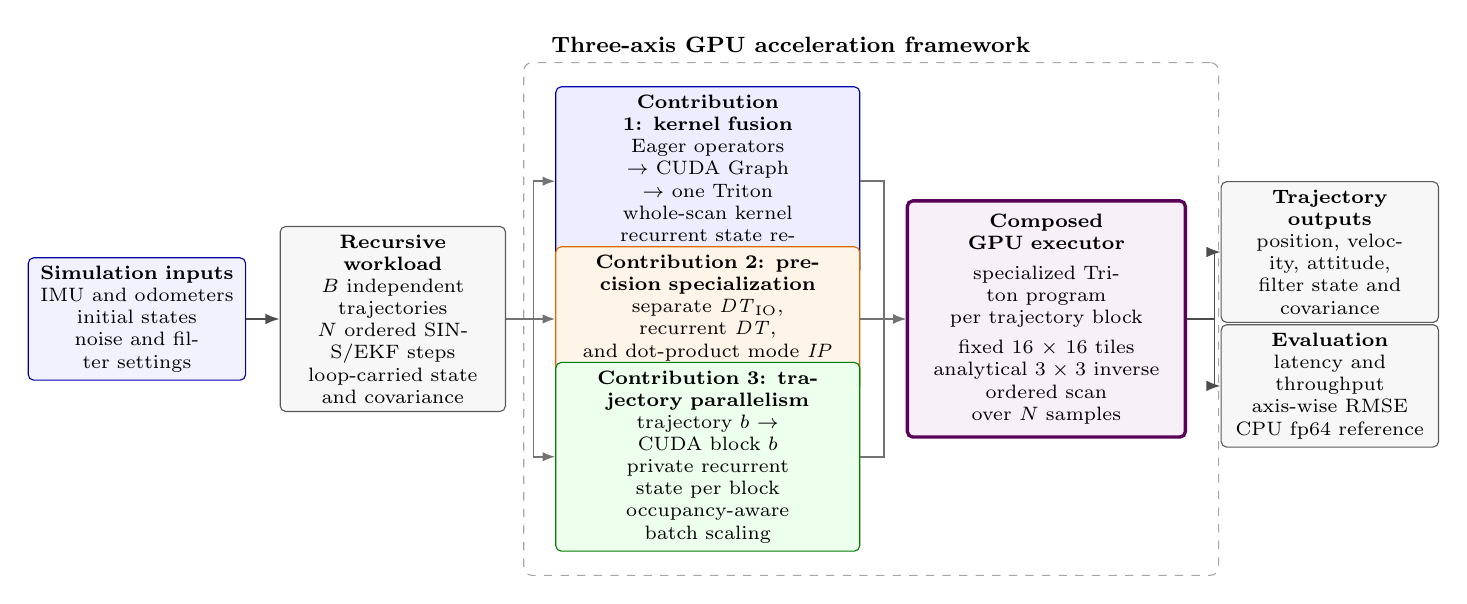
\begin{tikzpicture}[
      font=\scriptsize,
      input/.style={draw=blue!65!black, rounded corners=2pt,
        fill=blue!5, align=center, text width=2.55cm,
        minimum height=12mm, inner sep=3pt},
      workload/.style={draw=black!65, rounded corners=2pt,
        fill=black!3, align=center, text width=2.65cm,
        minimum height=14mm, inner sep=3pt},
      fusion/.style={draw=blue!70!black, rounded corners=2pt,
        fill=blue!7, align=center, text width=3.65cm,
        minimum height=12mm, inner sep=3pt},
      precision/.style={draw=orange!85!black, rounded corners=2pt,
        fill=orange!9, align=center, text width=3.65cm,
        minimum height=12mm, inner sep=3pt},
      parallel/.style={draw=green!50!black, rounded corners=2pt,
        fill=green!7, align=center, text width=3.65cm,
        minimum height=12mm, inner sep=3pt},
      executor/.style={draw=violet!70!black, very thick, rounded corners=2pt,
        fill=violet!6, align=center, text width=3.25cm,
        minimum height=30mm, inner sep=4pt},
      output/.style={draw=black!65, rounded corners=2pt,
        fill=black!3, align=center, text width=2.55cm,
        minimum height=12mm, inner sep=3pt},
      arrow/.style={-{Latex[length=1.8mm]}, semithick, draw=black!70},
      link/.style={-{Latex[length=1.6mm]}, semithick, draw=black!55}
    ]
    \node[input] (inputs) at (0,0)
      {\textbf{Simulation inputs}\\IMU and odometers\\initial states\\noise and filter settings};
    \node[workload] (scan) at (3.25,0)
      {\textbf{Recursive workload}\\$B$ independent trajectories\\$N$ ordered SINS/EKF steps\\loop-carried state and covariance};

    \node[fusion] (fusion) at (7.25,1.75)
      {\textbf{Contribution 1: kernel fusion}\\Eager operators $\rightarrow$ CUDA Graph\\$\rightarrow$ one Triton whole-scan kernel\\recurrent state retained on chip};
    \node[precision] (precision) at (7.25,0)
      {\textbf{Contribution 2: precision specialization}\\separate $\mathit{DT}_{\mathrm{IO}}$, recurrent $\mathit{DT}$,\\and dot-product mode $\mathit{IP}$\\compile-time kernel variants};
    \node[parallel] (parallel) at (7.25,-1.75)
      {\textbf{Contribution 3: trajectory parallelism}\\trajectory $b$ $\rightarrow$ CUDA block $b$\\private recurrent state per block\\occupancy-aware batch scaling};

    \node[executor] (executor) at (11.55,0)
      {\textbf{Composed GPU executor}\\[1mm]
       specialized Triton program\\per trajectory block\\[1mm]
       fixed $16\times16$ tiles\\analytical $3\times3$ inverse\\ordered scan over $N$ samples};

    \node[output] (outputs) at (15.15,0.85)
      {\textbf{Trajectory outputs}\\position, velocity, attitude,\\filter state and covariance};
    \node[output] (validation) at (15.15,-0.85)
      {\textbf{Evaluation}\\latency and throughput\\axis-wise RMSE\\CPU fp64 reference};

    \draw[arrow] (inputs) -- (scan);
    \draw[link] (scan.east) -- ++(0.35,0) |- (fusion.west);
    \draw[link] (scan.east) -- (precision.west);
    \draw[link] (scan.east) -- ++(0.35,0) |- (parallel.west);
    \draw[link] (fusion.east) -- ++(0.30,0) |- (executor.west);
    \draw[link] (precision.east) -- (executor.west);
    \draw[link] (parallel.east) -- ++(0.30,0) |- (executor.west);
    \draw[arrow] (executor.east) -- ++(0.35,0) |- (outputs.west);
    \draw[arrow] (executor.east) -- ++(0.35,0) |- (validation.west);

    \node[draw=black!35, dashed, rounded corners=3pt,
      fit=(fusion)(precision)(parallel)(executor),
      inner xsep=4mm, inner ysep=3mm] (framework) {};
    \node[font=\footnotesize\bfseries, anchor=south west,
      fill=white, inner xsep=1.5mm]
      at ([xshift=2mm]framework.north west) {Three-axis GPU acceleration framework};
  \end{tikzpicture}
  \caption{Design overview of the proposed GPU acceleration framework. The recursive SINS/EKF workload is transformed along three complementary axes: whole-scan kernel fusion reduces launch and state-traffic overhead, component-aware precision specialization balances numerical stability and hardware cost, and multi-trajectory mapping exposes block-level parallelism. The three transformations are composed in one GPU executor and validated against the CPU fp64 reference.}
  \label{fig:design-overview}
\end{figure*}

\subsection{From Fragmented Operators to a Fused Recursive Scan}
\label{subsec:kernel-fusion}

The fusion path has three stages that progressively enlarge the optimization scope. The first stage rewrites scalar tensor construction, host-visible scalar access, and dynamic concatenation as device-side tensor expressions. It also replaces the two possible observation shapes with one fixed three-dimensional representation. When the odometry consistency test rejects the displacement observation, its variance is set to a sufficiently large value, causing the corresponding Kalman gain to approach zero while retaining a static matrix shape. This stage produces a compile-friendly EKF step with fixed control flow and storage dimensions.

The second stage captures the fixed-shape step in a CUDA Graph and replays it for the sensor sequence. Graph replay reduces repeated host dispatch, but the device still executes the fine-grained kernels contained in the captured step and transfers recurrent values between them. We retain this stage as an intermediate design point because it separates host launch overhead from device-side fragmentation.

The final stage expresses the complete $N$-step scan as one Triton kernel. A single Triton program processes one trajectory and executes the time loop in program order. At iteration $k$, it loads only the current gyroscope, accelerometer, and odometer samples; updates the quaternion, velocity, and position; constructs the transition and observation operators; propagates the error state and covariance; and applies the EKF feedback. The position, velocity, quaternion, error state, and covariance remain program-local across iterations, eliminating intermediate tensors and recurrent-state round trips to global memory. Only the requested trajectory outputs are stored after each step.

Two transformations make the fused kernel static and self-contained. First, the logical filter matrices are padded to $16\times16$ and accessed with masks, allowing a common tile layout for transition, covariance, observation, and gain products while retaining the original 15-state semantics. Second, the $3\times3$ innovation covariance is inverted through its adjugate and determinant inside the kernel. This avoids invoking a general solver on the critical path and permits graph capture and whole-scan fusion without a host synchronization point. The fused design preserves the unavoidable temporal order and uses locality to shorten its sequential critical path.

\subsection{Component-Aware Precision Specialization}
\label{subsec:mixed-precision}

Uniform precision assigns the same cost and error behavior to values with different numerical roles. In this workload, sensor samples are noisy external inputs, whereas position, velocity, attitude, and covariance are recurrent quantities whose rounding errors can accumulate over the full trajectory. Small matrix products introduce a third choice because TensorFloat-32 changes the multiplication path independently of the storage type. We therefore separate input precision, recurrent computation precision, and dot-product precision.

The kernel exposes three compile-time parameters. $\mathit{DT}_{\mathrm{IO}}$ controls the precision used when loading IMU and odometer samples. The samples are immediately converted to the internal type $\mathit{DT}$, which is used for quaternion normalization, SINS integration, EKF state propagation, covariance update, and feedback. The parameter $\mathit{IP}$ selects the input mode of Triton dot products, allowing IEEE arithmetic and TensorFloat-32 paths to be evaluated without changing the surrounding kernel. All three parameters are declared as compile-time constants, so every combination generates a specialized kernel and introduces no precision-selection branch in the recursive loop.

\begin{table}[!t]
  \centering
  \caption{Precision dimensions exposed by the fused implementation.}
  \label{tab:precision-design}
  \begin{tabular}{@{}lll@{}}
    \toprule
    Component & Candidate & Treatment \\
    \midrule
    Sensor input & fp16, bf16, fp32 & cast to $\mathit{DT}$ \\
    Recursive computation & fp32, fp64 & retain across steps \\
    Small matrix products & IEEE, TF32 & $\mathit{IP}$ specialization \\
    Validation reference & fp64 & CPU trajectory \\
    \bottomrule
  \end{tabular}
\end{table}

Candidate configurations are screened over the complete trajectory instead of isolated filter steps. A configuration is considered numerically acceptable when its accumulated state deviation remains small relative to both the fp64 reference and the positioning error caused by the simulated sensing and motion models. This policy captures failures that appear only after repeated integration or covariance propagation. It also keeps hardware behavior separate from numerical acceptance: reduced storage, reduced arithmetic precision, and Tensor Core execution are measured as distinct choices rather than being grouped under a single mixed-precision label.

\subsection{Multi-Trajectory Batch Parallelism}
\label{subsec:batch-parallelism}

A fused scan for one trajectory occupies one CUDA block and offers little parallel work to the remaining SMs. Simulation campaigns, however, commonly evaluate multiple noise seeds, obstacle arrangements, or filter parameters. These trajectories have the same computational structure and share no recursive state. For a batch size $B$, we launch a one-dimensional grid of $B$ blocks and assign trajectory $b$ to program identifier $b$. Every input and output address is computed as
\begin{equation}
  \operatorname{addr}(b,k)=\operatorname{base}+b\,s_B+k\,s_N,
  \label{eq:batch-address}
\end{equation}
where $s_B$ and $s_N$ are the trajectory and time strides. Program-local SINS and EKF values are initialized independently for each block; no synchronization or communication is required between trajectories.

The mapping also gives a simple resource-based scaling model. Let $S$ denote the number of SMs, $R_{\mathrm{SM}}$ the registers available per SM, and $R_{\mathrm{blk}}$ the register allocation of one trajectory block. Ignoring other limits, the maximum number of resident trajectory blocks per SM is
\begin{equation}
  C_{\mathrm{reg}}=\left\lfloor
  \frac{R_{\mathrm{SM}}}{R_{\mathrm{blk}}}\right\rfloor,
  \qquad B_{\mathrm{sat}}\approx S C_{\mathrm{reg}}.
  \label{eq:batch-saturation}
\end{equation}
For $B\leq S$, different trajectories can be placed on different SMs and aggregate throughput is expected to grow nearly linearly. For $S<B\leq B_{\mathrm{sat}}$, multiple blocks reside on an SM and increasingly compete for registers and execution resources. Beyond $B_{\mathrm{sat}}$, additional blocks execute in waves, so a larger batch need not improve instantaneous throughput. The model connects the algorithmic batch dimension to observable hardware limits and is tested with the batch-size sweep in \Cref{subsec:batch-evaluation}.

\section{Evaluation}
\label{sec:evaluation}

\subsection{Experimental Setup}
\label{subsec:experimental-setup}

Experiments use an NVIDIA Hopper GPU with 78 SMs, PyTorch 2.11.0, CUDA 12.9, and Triton 3.6.0. The principal dataset contains 166,667 samples. The CPU eager fp64 implementation is used as the numerical golden reference. Reported GPU timings exclude compilation and use warm-up runs with the same problem shape as the measured execution. Throughput is reported in processed filter steps per second and, for batch experiments, trajectories per second.

% TODO: Add the exact GPU model, CPU model, memory configuration, driver,
% operating system, compiler flags, and number of repeated measurements.

\subsection{End-to-End Performance}
\label{subsec:end-to-end}

\begin{table}[!t]
  \centering
  \caption{End-to-end performance summary. The final manuscript will report means and variability over repeated runs.}
  \label{tab:end-to-end}
  \begin{tabular}{@{}llrr@{}}
    \toprule
    Version & Method & Steps/s & Speedup \\
    \midrule
    v0 & CPU eager fp64 & 1,866 & 1.0$\times$ \\
    v2 & CUDA Graph fp64 & 2,640 & 1.41$\times$ \\
    v3 & Triton fused fp64 & 16,491 & 8.8$\times$ \\
    v4 & Triton fused fp32 & 242,737 & 130$\times$ \\
    v5 & fp32, batch 78 & 17.8--19.1M & approx. 10,000$\times$ \\
    v7 & fp32, batch 312 & 46.3M & approx. 24,800$\times$ \\
    \bottomrule
  \end{tabular}
\end{table}

This subsection will separate latency improvements for one trajectory from aggregate throughput improvements for batches. It will also reconcile performance values from different experiment rounds using the archived JSON results as the final source of truth.

\subsection{Effect of Kernel Fusion}
\label{subsec:fusion-evaluation}

This subsection will compare eager execution, compile-friendly restructuring, CUDA Graph replay, and the Triton mega-kernel. Profiler evidence will include kernel counts, launch intervals, time spent in solver calls, global-memory traffic, register use, and achieved SM throughput.

\subsection{Accuracy and Precision Trade-offs}
\label{subsec:precision-evaluation}

The precision study will report throughput together with final-state deviation and X/Y/Z RMSE. The main comparison includes fp64, fp32, TensorFloat-32 matrix products, fp16 sensor input, and bfloat16 variants. Negative results are retained because they identify when reduced precision is unsafe in a long recursive filter.

\subsection{Batch Scalability and Resource Saturation}
\label{subsec:batch-evaluation}

Batch sizes from one trajectory to beyond the register-limited residency point will be evaluated. The analysis will distinguish the linear region up to 78 blocks, the resource-contention region, and the saturation region around 312 blocks. Nsight Compute metrics will be used to connect the observed boundaries to register pressure and active blocks per SM.

\subsection{Ablation and Negative Results}
\label{subsec:ablation}

The ablation study will isolate fusion, precision, and batch parallelism. Additional experiments will document the limited value of TensorFloat-32, CUDA streams for uniform trajectories, Tensor Memory Accelerator usage, warp specialization, and conventional tile or layout auto-tuning. These results support the claim that the optimization space of latency-bound micro-matrix recursion differs from that of large dense linear algebra.

\section{Related Work}
\label{sec:related-work}

\subsection{Downhole Tractors and In-Pipe Robots}
\label{subsec:related-downhole}

Recent field studies demonstrate that downhole tractors can convey wireline tools and support intervention, logging, and perforation in highly deviated and horizontal wells~\cite{he2020downhole-tractor,chawla2024tractor-glide}. Existing work primarily addresses traction capability, tool conveyance, and operational reliability. Our work complements it by studying the computational behavior of long-horizon multi-sensor positioning simulation and by optimizing its recursive SINS/EKF workload for GPU execution.

\subsection{GPU-Accelerated Kalman Filtering}
\label{subsec:related-kalman}

GPU implementations of Kalman filtering expose parallelism at several different levels. Early work mapped the matrix operations within a filter step to CUDA and reported speedups when the matrices were large enough to amortize data movement and kernel-launch costs~\cite{huang2011gpu-kalman}. Application-specific systems more often exploit independent estimation problems. The GPU track-fitting implementation of Ai et al.~\cite{ai2021gpu-kalman} processes many particle tracks concurrently, while FastTrack parallelizes the prediction and update of multiple tracked objects and integrates the filter with the surrounding tracking pipeline~\cite{liu2024fasttrack}. These designs are effective when a workload supplies many simultaneous filters, although they do not remove the recurrence or fine-grained execution overhead of one long, small-state trajectory.

Another line of work derives temporally parallel filtering and smoothing algorithms. S\"arkk\"a and Garc\'ia-Fern\'andez formulate Bayesian smoothing operations as associative elements, enabling prefix-scan algorithms with logarithmic span~\cite{sarkka2021temporal}. Such reformulations are attractive when the model admits associative composition and parallel latency is the primary goal. The downhole traction robot positioning simulation studied here retains the original nonlinear SINS propagation, measurement selection, error feedback, and covariance recursion in their program order. We shorten this sequential path by fusing the complete scan and keeping its recurrent state local, then use independent simulation trajectories---rather than time steps from one trajectory---to occupy the GPU.

\subsection{MegaKernel and Kernel Fusion}
\label{subsec:related-fusion}

Kernel fusion combines operations so that intermediate values can remain on chip and repeated kernel launches can be avoided. MegaKernels enlarge this scope to a substantial computation region; for example, Jia et al.~\cite{jia2020megakernels} place the stages of fast convolution in one GPU kernel to reuse intermediate data and reduce launch and synchronization overhead. Recent compiler and systems research has extended fusion beyond manually selected, memory-bound operator chains. Welder constructs a tile graph to jointly search fusion and tile schedules according to memory traffic~\cite{shi2023welder}. Chimera uses an analytical model to select fusion plans for compute-intensive operators~\cite{zheng2023chimera}, and MCFuser combines memory-bound operators with compute-intensive operators while controlling recomputation and synchronization costs~\cite{zhang2024mcfuser}. These systems show that profitable fusion depends on both the operator graph and the hardware cost created by a candidate fused region.

More recent systems search larger transformation spaces. Mirage represents tensor programs at kernel, thread-block, and thread levels, allowing its superoptimizer to combine algebraic transformations, schedules, and custom-kernel generation~\cite{wu2025mirage}. STOF uses compilation templates and a two-stage search to select adaptive fusion strategies for sparse Transformer inference~\cite{dai2026stof}. These approaches primarily optimize tensor graphs whose operators retain substantial spatial parallelism. Our target presents a different fusion boundary: a complete sequential SINS/EKF trajectory is compiled as one Triton program~\cite{triton}, and its small navigation state and covariance remain program-local across time steps. Parallelism is recovered across independent trajectories, while fusion reduces the latency of each recurrent scan. This specialization complements graph-level fusion systems by addressing a long-lived kernel with an unavoidable loop-carried dependency.

\subsection{Mixed Precision for Scientific Computing}
\label{subsec:related-precision}

Mixed-precision methods have been widely studied in scientific computing and GPU acceleration~\cite{abdelfattah2021survey}. Baboulin et al.~\cite{mixed-precision} combine lower-precision kernels with higher-precision residual evaluation and correction in numerical linear algebra. Haidar et al.~\cite{haidar2018tensorcores} further map low-precision factorization and solves to GPU Tensor Cores while retaining higher precision for accuracy-critical operations.

Automatic precision selection provides a complementary approach. Precimonious searches variable- and operation-level assignments under an application-provided error constraint~\cite{rubio2013precimonious}. CoMP performs operator-wise precision selection for neural-network training through convergence-aware and performance-oriented sampling~\cite{dai2025comp}. Its search also considers format-conversion overhead and the availability of Tensor Core execution, illustrating the importance of evaluating precision plans against both numerical requirements and the characteristics of the target GPU.

\section{Conclusion}
\label{sec:conclusion}

This paper presents a three-axis approach to GPU acceleration of SINS/EKF fusion positioning for downhole traction robots. The central observation is that the workload is limited by launch latency, sequential dependency, and idle SMs rather than by arithmetic throughput. Whole-scan kernel fusion removes fragmented execution, component-aware precision matches numerical requirements to GPU hardware, and multi-trajectory mapping exposes the independent work needed to fill the device. The resulting implementation changes a naive GPU slowdown into substantial single-trajectory acceleration and scalable batch throughput while preserving positioning accuracy. Future work will evaluate the framework across additional state-estimation models, trajectory distributions, and GPU architectures, and will investigate structure-aware reductions in covariance computation.

\fontsize{8.5pt}{10pt}\selectfont

\section*{Acknowledgements}
% TODO: Add funding projects, facilities, and individual contributions.
To be completed.

\section*{Competing interests}
The authors declare that they have no competing interests or financial conflicts to disclose.

\bibliographystyle{fcs}
\bibliography{references}

% TODO: Add author biographies and high-resolution photographs after the
% author list has been finalized.

\end{document}
